\section{GK Model}

We compare the preliminary cross section to the model developed by S.V. Goloskokov and P. Kroll \cite{Goloskokov2010AnElectroproduction}. This model uses the handbag model to produce theoretical curves for specified sets of kinematic points. This model was implemented in the PARTONS framework \cite{Berthou2018PARTONS:Software} and was also used in the published CLAS6 result to compare with their experimental cross section, reproduced below in figure \ref{fig:oldres} \cite{Bedlinskiy2014ExclusiveCLAS}

As discussed, the \xsec for this process can be expressed in terms of structure functions as 

    \begin{equation*}
         \recallLabel{eq:DVPiPCrossSection_theory}
    \end{equation*}

\section*{Notes on GK model from Kemal:}

Thank you very much for your response. I include two short responses, below, as well as a third response/question that I hope you can read and respond to: 

\begin{itemize}
    \item Thank you for the reference about the Mandelstam function. I was afterwards able to also find reference to it here, where it was named Kallen Function. I haven't heard of either names before. Thanks! \href{https://en.wikipedia.org/wiki/K%C3%A4ll%C3%A9n_function}{Källén Function on Wikipedia}

    \item Yes, I am using the code for $\pi^0$, so I do not believe any changes need to be made. I am just working from the single C++ file, since it is easier than getting set up with a full partons framework which looked like it had some overhead to setup and install.
\end{itemize}

\textbf{Important question:} I now understand that you took the most updated parameters from P Kroll that would best describe the JLab kinematics from the 2020 paper, and that these are different from the parameters available in 2013. My question to you is - are the parameters that are currently implemented in the GK model the best parameters for me to use (for calculating $\pi^0$ cross section at JLab CLAS12 10.6 GeV experiment)? Do you take into account any other experiments (such as work in hall A or C) for finding the parameters? To say it differently, how are optimal parameters chosen for this model?

I would refrain myself speaking on behalf of the authors on that question. They might give you better insights into their model. But I can tell you my viewpoint. I think the GPDs should not be optimized for your data. What I mean is the following: since GPDs are universal functions, ideally there should not be multiple parameters for different experiments (so that we have the flexibility to choose among different parameter sets). Rather, the more data we get, the better parameters need to be determined and those parameters need to be unique for all experiments. In this regard, I would just use the latest parameters that the authors offer (assuming that they did a global analysis to tune those parameters). You could alternatively try to change the parameters to fit them to your data and suggest how your data will impact the extraction of the parameters.

I hope it makes sense, otherwise, we could discuss it further.

Sorry for the late reply. During the last few weeks, I had some other tasks to complete. I'll be happy to share my thoughts with you.

\begin{enumerate}
    \item I think the difference is just the different parameters used in separate works. The parameters of GPDs and their t-slope are not completely the same. At the time I wrote the code, I took the most updated parameters from P. Kroll (or parameters that he thought would best describe the JLab kinematics in Fig. 3 of \href{https://arxiv.org/pdf/2007.15677.pdf}{this paper}). So, I would not expect the same curves just because the GPDs in those works have different parameters.

    \item The function $\Lambda$ is called the Mandelstam variable and somehow I could not find the generic expression online. But, I expressed the definition in my thesis (see Eq. 4.50 on page 129); \href{https://www.osti.gov/biblio/1881460}{this link} therein (Chapter 4) you can also see a more detailed implementation of the model. The value of 0.3894 comes from the conversion from $\text{GeV}^{-2}$ to mb.

    \item Yes, the final code works for both $\pi^+$ and $\pi^0$ (I am not sure which one you use; if you use the one that you shared above, then it would work only for $\pi^0$. $\pi^+$ implementation can be found in the PARTONS v3. or I have the code for $\pi^+$ similar to the $\pi^0$ that you shared above). Their formulation is quite similar albeit with important differences. First of all, the $\pi^0$ production does not include the so-called pion-pole contribution (see Eq. 4.39 - 4.42 in my thesis). Moreover, their handbag contributions are slightly different. Their differences at the handbag level are discussed in Eq. 4.37 and 4.38 in my thesis.
\end{enumerate}

Just let me know if you need any further clarification; I'll be happy to address it.







\begin{figure}[hbt]
	\centering
	\includegraphics[page=6,width=0.6\linewidth]{Chapters/Ch5-Further/GK_model/pics/clas6comp.jpg}
\end{figure}\label{fig:oldres}

To validate the model, we ran the implementation to generate curves and compared to the published CLAS6 result. We observed that the sigma T and sigma L terms were comparable, but not exactly the same, as the 2014 published results, while the sigma TT term was significantly different. It is believed that these differences are due to improvements in the model made in the past 8 years. Figure \ref{fig:oldres2} shows one example bin of this comparison, where the color of the curves is matched to the corresponding color of the structure functions.


The parameters for the GK model were taken from 

$
Their formulation is quite similar albeit with important differences. First of all, the pi0 production does not include the so-called pion-pole contribution (see Eq. 4.39 - 4.42 in my thesis). Moreover, their handbag contributions are slightly different. Their differences at the handbag level are discussed in Eq. 4.37 and 4.38 in my thesis. $

The parameters of GPDs and their t-slope are not completely the same. At the time I wrote the code, I took the most updated parameters from P. Kroll (or parameters that he thought would best describe the JLab kinematics in Fig. 3 of \cite{Diehl2020ExtractionKinematics} ). So, I would not expect the same curves just because the GPDs in those works have different parameters. 

Lambda is defined as: %$https://en.wikipedia.org/wiki/Källén_function$

Description of GK by Kemal Thesis:

The Goloskokov-Kroll model has been phenomenologically successful (inlcude links showing this).  The description is based on QCD factorization theorems. In factorizable processes, the amplitudes can be written as a convolution of a hard scattering which is computable in pQCD, and a soft non perturbative part parameterized by GPDs. Chiral-even GPDs are accessible through DVCS where factorization was proven (CITE). Chiral-odd GPDs can be accessed at subleading twist through Deeply Virtual Meson Production if one assumes an effective handbag mechanism, as descried by the GK model. 
QCD factorization theorem for DVMP process has only been proven for longitudinally polarized photons, and also that the cross section is suppressed by a power of 1/Q for transversley polarized photons. 
The GK model computes contributions from transversely polarized photons in the handbag mechanism as a twist-3 effect in which teh soft part of the process is parameterized in terms of Chiral Odd GPDs.
Several GK model parameters implemented in teh PARTONS framework differ from teh parameters used in refrences. The GK model parameters implemented are used in two different publicatoins
The GK model, under the assumption of flavor-symmetric sea GPDs, only valence quark GPDs Htilda Etilda Ht and Etildat are needed to describe teh process in the kinematical region of large Q2 but small zai and t. GPDs in teh GK model are constructed from double distribtuions as follows, which can be integrated analytically, and the GPDs can be expressed in teh following form:


From Easy as Pi:
Among the many important consequences is the fact that differently from both inclusive and semi-inclusive processes, GPDs can in principle provide essential information
for determining the missing component to the nucleon longitudinal spin sum rule, which
is identified with orbital angular momentum. A complete description of nucleon structure
%requires, however, also the transversity (chiral odd/quark helicity-flip) GPDs, HT (x, ξ, t),
%ET (x, ξ, t), HeT (x, ξ, t), and EeT (x, ξ, t) [1]. J


\begin{figure}[hbt]
	\centering
	\includegraphics[page=6,width=0.6\linewidth]{Chapters/Ch5-Further/GK_model/pics/2022_vs_2014_GK_model.jpg}
\end{figure}\label{fig:oldres2}

Finally, we compare the preliminary CLAS12 reduced cross section to the predictions from the GK model. Sample plots are shown below. Agreement is close but not exact. The functional form is as expected. It is unclear if the offset between the CLAS12 fit and the GK model is due to a model discrepancy, or an absolute normalization uncertainty in the CLAS12 calculation. More quantitative statments will be made when uncertainties and correction factors in the CLAS12 work are better understood.
\begin{figure}[hbt]
	\centering
	\includegraphics[page=6,width=0.45\linewidth]{Chapters/Ch5-Further/GK_model/pics/reduced_xsec_1.5_2_0.2_0.25_0.2_0.3.png}
	\includegraphics[page=6,width=0.45\linewidth]{Chapters/Ch5-Further/GK_model/pics/reduced_xsec_1.5_2_0.25_0.3_0.2_0.3.png}
\end{figure}\label{fig:oldres4}



